% TODO: The bibfile is very wrong in citing everything (webpages, chapters of a page, etc) as @article -- fix it

\documentclass[a4paper]{amsart}

\usepackage{textcomp}
\usepackage{amsmath}
\usepackage{amsthm}
\usepackage{amsfonts}
\usepackage{amssymb}
\usepackage{hyperref}
\usepackage{cleveref}
\usepackage{enumitem}
\usepackage{svg}
\usepackage{float}
\usepackage{xcolor}
\usepackage{tkz-base}
\usepackage{subfig}

\theoremstyle{plain}
\newtheorem{theorem}{Theorem}
\newtheorem{lemma}{Lemma}
\newtheorem{corollary}{Corollary}
\newtheorem{remark}{Remark}
\theoremstyle{definition}
\newtheorem{definition}{Definition}

\floatplacement{figure}{h}

\begin{document}

\title{\(n^2 + 1\) unit equilateral triangles cannot cover an equilateral triangle of side \(> n\) if all triangles have parallel sides}

\author{Jineon Baek*}
\thanks{*University of Michigan - Ann Arbor, \texttt{jineon@umich.edu}}
\author{Seewoo Lee**}
\thanks{**University of California - Berkeley, \texttt{seewoo5@berkeley.edu}}

\begin{abstract}
\textcolor{red}{Draft. DO NOT DISTRIBUTE.}
In a famous short paper, Conway and Soifer asked if an equilateral triangle \(T\) of side \(n + \varepsilon\) with sufficiently small \(\varepsilon > 0\) can be covered by \(n^2 + 1\) unit equilateral triangles, and provided two ways to cover \(T\) with \(n^2 + 2\) unit triangles. We show that if we require the sides of all triangles to be parallel to the sides of \(T\) (e.g. $\bigtriangleup$ and $\bigtriangledown$), then it is impossible to cover \(T\) with exactly \(n^2 + 1\) unit equilateral triangles.
\end{abstract}

\maketitle

\section{Introduction}

In 2004, Conway and Soifer attempted to set a world record in the minimum number of words in a paper by submitting the following paper to the \emph{American Mathematical Monthly} \cite{soifer2009coffee}.
\\
\begin{quote}
\begin{center}
\Large \textbf{Can \(n^2 + 1\) unit equilateral triangles cover an equilateral triangle of side \(> n\), say \(n + \varepsilon\)?\footnote{Reproduction done by authors with slight modification; for the exact we refer to \cite{soifer2009coffee}.}}
\end{center}

\begin{center}
John H. Conway \& Alexander Soifer
\end{center}

\(n^2 + 2\) can:
\begin{figure}[h]
   \begin{minipage}{0.5\textwidth}
     \centering
     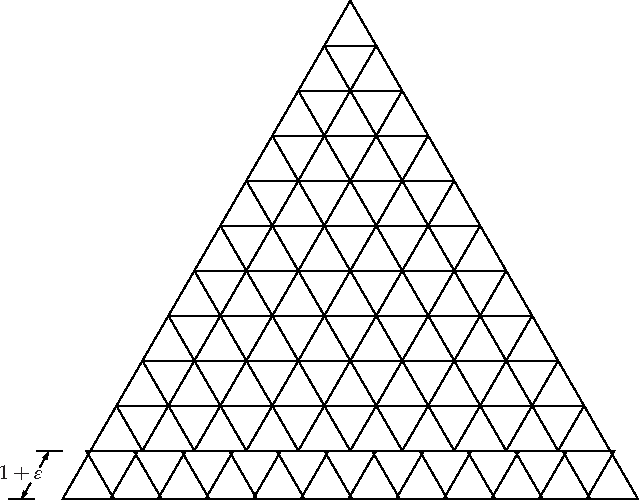
\includegraphics[width=0.9\linewidth]{triangle1.pdf}
     \caption{}
     \label{fig:triangle1}
   \end{minipage}\hfill
   \begin{minipage}{0.5\textwidth}
     \centering
     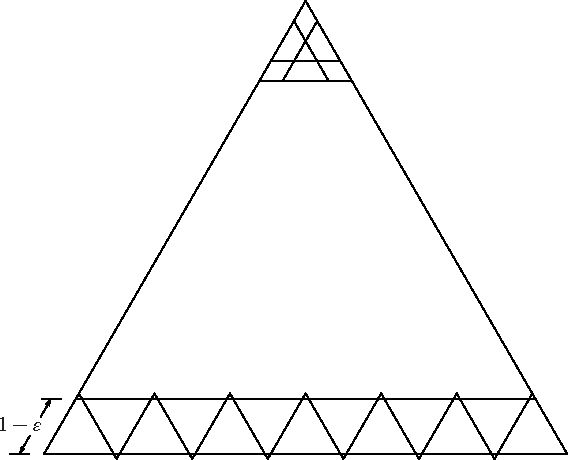
\includegraphics[width=0.9\linewidth]{triangle2.pdf}
     \caption{}
     \label{fig:triangle2}
   \end{minipage}
\end{figure}
\end{quote}
The \emph{American Mathematical Monthly} didn't publish the paper as-is and instead put it inside a ``boxed filler'' with modifications \cite{conway2005covering},
but the paper is often mentioned as an example of mathematics papers with shortest length in multiple places (e.g. blogs \cite{ShortestKnownPaperPublished, ShortestPapersEver}, online communities \cite{bhuyanWhatShortestPaper2015, creinaldoShortestPaperEver2015, hellon00bShortestKnownPaperPublished2015}, and a Numberphile video).

Related, Karabash and Soifer showed that for every non-equilateral triangle \(T\), \(n^2 + 1\) triangles similar to \(T\) and with the ratio of linear sizes \(1: (n + \varepsilon)\), can cover \(T\) \cite{karabash2005covering}. 
Also, they generalized the result of Conway and Soifer and showed that a \emph{trigon}\footnote{A connected shape formed by unit equilateral triangles with matching edges.} made of \(n\) unit equilateral triangles can be covered by \(n + 2\) triangles of side \(1 - \varepsilon\) \cite{karabash2005covering}.
A similar problem of covering a square of side \(n + \varepsilon\) with unit squares has been also extensively studied \cite{karabash2006sharp, karabash2008note, chung2009packing, wang2016new, chungEfficientPackingsUnit2020}.
Still, to the best of the authors' knowledge, the original question in the title of the paper by Conway and Soifer haven't been addressed in the literature.

Define an equilateral triangle as \emph{upright} if all the sides of the triangle are parallel to the three axes of a triangular grid.
Note that both triangles $\bigtriangleup$ and $\bigtriangledown$ are upright, and all the unit triangles used in Figure 1 and 2 are upright.
Also, the generalized covering of trigons by Karabash and Soifer \cite{karabash2005covering} only uses upright triangles as well.
Thus, it is natural to ask if one can cover the equilateral triangle of side \(> n\) with \(n^2 + 1\) upright unit triangles.
In this paper, we settle this problem by showing that such covering with upright unit triangles does not exist.

The proof generalizes to an arbitrary union \(X\) of \(n\) upright triangles with disjoint interiors: it is impossible to cover \(X\) with \(n + 1\) equilateral triangles of side \(< 1\).

\begin{theorem}

Let \(X\) be any union of \(n\) unit upright equilateral triangles \(S_1, S_2, \dots, S_n\) with disjoint interiors. Then \(X\) cannot be covered by \(n + 1\) upright equilateral triangles of sides less than one.

\label{thm:triangle-cover}
\end{theorem}

To recover the original problem, assume that an upright equilateral triangle \(T\) of side \(> n\) can be covered by \(n^2 + 1\) unit upright equilateral triangles. Rescale the covering so that \(T\) have side \(n\) and the small triangles have side \(< 1\). Then we get contradiction by \Cref{thm:triangle-cover} as \(T\) is a union of \(n^2\) unit triangles with disjoint interiors.

\begin{corollary}

\(n^2 + 1\) unit upright equilateral triangles cannot cover an upright equilateral triangle of side \(> n\).

\label{cor:triangle-cover}
\end{corollary}

With the covering of \(T\) by Conway and Soifer (\Cref{fig:triangle1} and \ref{fig:triangle2}), and the covering of trigons by Karabash and Soifer,
we match the exact minimum number of upright unit equilateral triangles for covering.

\begin{corollary}

The minimum number of unit upright equilateral triangles required to cover an upright equilateral triangle of side \(> n\) is exactly \(n^2+2\). Also, the minimum number of unit upright triangles required to cover a trigon of \(n\) triangles is exactly \(n + 2\).

\label{cor:triangle-cover-number}
\end{corollary}

\section{Proof of \Cref{thm:triangle-cover}}

Take the standard Cartesian \(xy\)-coordinate system of a plane. Inside the plane, take the triangular grid of unit equilateral triangles with the \(x\)-axis as one of the three axes of the triangular grid.

For every unit upright triangle \(T\), define its rescaled \(y\)-coordinate \(z_T\) as the \(y\)-coordinate of the horizontal side of $T$ divided by \(\sqrt{3}/2\). Note that \(\sqrt{3}/2\) is the height of a unit equilateral triangle, so the value of \(z_T\) is an integer for every triangle \(T\) in the triangular grid.
Define the function \(\tilde{f}_T : \mathbb{R} \to \mathbb{R}\) as the following. For any \(z \neq z_T\), the value \(\tilde{f}_T(z)\) is the length of the part of the line \(y = \sqrt{3}z / 2\) covered by triangle \(T\) (the value is zero if \(T\) is disjoint from the line). The value of \(\tilde{f}_T(z_T)\) is chosen so that \(\tilde{f}_T\) is right-continuous everywhere: 1 if \(T\) is pointed upwards, and 0 if \(T\) is pointed downwards.

In this paper, let \(S^1\) be the abelian group quotient \(\mathbb{R} /\mathbb{Z}\). For every unit upright triangle \(T\), define \(f_T : S^1 \to \mathbb{R}\) as the function \(f_T(t + \mathbb{Z}) = \sum_{n \in \mathbb{Z}} \tilde{f}_T(t + n)\).
For every \(a \in S^1\), define \(\tilde{a} \in [0, 1)\) as the unique representator of \(a\) in the interval \([0, 1)\). Define \(\nabla (x) = \tilde{x}\) for all \(x \in S^1\). Define \(\Delta_0 (0) = 1\) and \(\Delta_0(x) = 1 - \tilde{x}\) for all nonzero \(x \in \mathbb{R}/\mathbb{Z}\). For every \(a \in S^1\), define the functions \(\Delta_a , \nabla_a : S^1 \to \mathbb{R}\) as the functions \(\nabla_a(x) = \nabla_0(x-a)\) and \(\Delta_a(x) = \Delta_0(x-a)\). If an unit upright triangle \(T\) is pointed upwards, we have \(f_T = \Delta_{y_T}\), and if \(T\) is pointed downwards, we have \(f_T = \nabla_{y_T}\). 


\begin{figure}
  \centering
  \subfloat{
    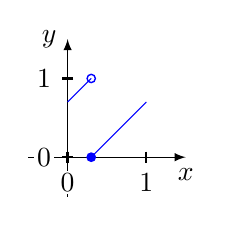
\begin{tikzpicture}
      \tkzInit[xmin = -0.5, xmax = 1, ymin = -0.5, ymax = 1]
      \tkzAxeXY
      \draw[blue] (0, 0.7) -- (0.3, 1);
      \draw[blue] (0.3, 0) -- (1, 0.7);
      \node [circle, draw, fill=none, line width = .5pt, color = blue, inner sep = 0pt, minimum size = 3pt] (ca) at (0.3, 1) {};
      \node [circle, draw, fill, line width = .5pt, color = blue, inner sep = 0pt, minimum size = 3pt] (ca) at (0.3, 0) {};
    \end{tikzpicture}
  }
  \qquad
  \subfloat{
    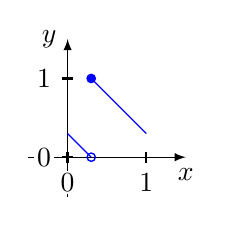
\begin{tikzpicture}
      \tkzInit[xmin = -0.5, xmax = 1, ymin = -0.5, ymax = 1]
      \tkzAxeXY
      \draw[blue] (0, 0.3) -- (0.3, 0);
      \draw[blue] (0.3, 1) -- (1, 0.3);
      \node [circle, draw, fill, line width = .5pt, color = blue, inner sep = 0pt, minimum size = 3pt] (ca) at (0.3, 1) {};
      \node [circle, draw, fill=none, line width = .5pt, color = blue, inner sep = 0pt, minimum size = 3pt] (ca) at (0.3, 0) {};
    \end{tikzpicture}
  }
  \label{fig:graph}
  \caption{Graphs of $\nabla_a(x)$ and $\Delta_a(x)$.}
\end{figure}


We now prove \Cref{thm:triangle-cover} by contradiction. Assume that the union \(X\) of \(n\) unit upright equilateral triangles \(S_1, S_2, \dots, S_n\) with disjoint interiors can be covered by \(n+1\) triangles \(T'_0, T'_1, \dots, T'_n\) of side \(< 1\). Take arbitrary \(n + 1\) triangles \(T_0, T_1, \dots, T_n\) of side 1 so that each \(T_i\) contains smaller triangle \(T_i'\).

Define \(\tilde{g} : \mathbb{R} \to \mathbb{R}\) as the function \(\tilde{g} = \sum_{i=0}^n \tilde{f}_{T_i} - \sum_{j=1}^n \tilde{f}_{S_j}\). Take any \(z\) different from the rescaled \(y\)-coordinates \(z_{T_i}\) and \(z_{S_j}\) of the triangles. As the triangles \(T_0, T_1, \dots, T_n\) cover the union \(X\) of disjoint triangles \(S_1, S_2, \dots, S_n\), the total length of the parts of the line \(y = \sqrt{3}z/2\) covered by \(T_i\)\textquotesingle s is at least the total length of the parts of the line \(y = \sqrt{3}z/2\) coverved by \(S_j\)\textquotesingle s. Thus we have \(\tilde{g}(z) \geq 0\). As \(\tilde{g}\) is right-continuous, by sending the right limit we have \(\tilde{g}(z) \geq 0\) for every \(z \in \mathbb{R}\) including the case where \(z\) is the rescaled \(y\)-coordinate of some triangle.

Define \(g : S^1 \to \mathbb{R}\) as \(g = \sum_{i=0}^n f_{T_i} - \sum_{j=1}^n f_{S_j}\) so that we have \(g(z + \mathbb{Z}) = \sum_{n \in \mathbb{Z}} \tilde{g}(z + n)\). Then consequently we have \(g(t) \geq 0\) for every \(t \in S^1\). 
It turns out that this is sufficient to derive a contradiciton.
Define \(\mathcal{T}\) as the abelian group generated by all functions \(\nabla_a , \Delta_a\) with \(a \in S^1\). Then \(g \in \mathcal{T}\) by the definition of \(g\).
We now examine the properties of $g \in \mathcal{T}$.
 
Denote the integral of any integrable function \(f : S^1 \to \mathbb{R}\) over the whole \(S^1\) as simply \(\int f\).
Say that two real numbers are equal modulo 1 if their difference is in $\mathbb{Z}$.

\begin{lemma}

Any function \(f : S^1 \to \mathbb{R}\) in \(\mathcal{T}\) has the following properties.

\begin{itemize}
\item
  \(f\) is right-continuous.
\item
  \(f\) is differentiable everywhere except for a finite number of points, and the derivative is equal to some fixed constant \(a \in \mathbb{Z}\).
\item
  For all \(x, y \in \mathbb{R}\), the value \(f(y + \mathbb{Z}) - f(x + \mathbb{Z})\) is equal to \(a(y - x)\) modulo 1.
\item
  The integral \(\int f\) is equal to \(b / 2\) for some \(b \in \mathbb{Z}\) where \(b - a\) is divisible by 2.
\end{itemize}

\label{lem:triangle-group}
\end{lemma}

\begin{proof}
Check that all the claimed properties are closed under addition and negation. Then check that the functions \(\nabla_a\) and \(\Delta_a\) with \(a \in S^1\) satisfies the claimed properties.
\end{proof}

We observed that \(g \in \mathcal{T}\) and \(g(t) \geq 0\) for every \(t \in S^1\). Also, for any unit upright triangle \(T\) we have \(\int f_T = 1/2\) so we also have \(\int g = 1/2\) by the definition \(g = \sum_{i=0}^n f_{T_i} - \sum_{j=1}^n f_{S_j}\). 
We now use the following lemma.
For any real number \(x\), let \(\left\{ x \right\}\) be the value in \([0, 1)\) equal to \(x\) modulo 1.

\begin{lemma}

Let \(f : S^1 \to \mathbb{R}\) be any function in \(\mathcal{T}\) such that \(\int f = 1/2\) and \(f(x) \geq 0\) for every \(x \in S^1\). Then there is a positive odd integer \(a\) and some \(c \in [0, 1)\) such that \(f\) is either \(f(x) = \left\{ ax + c \right\}\) or \(f(x) = 1 - \left\{ ax + c \right\}\).

\label{lem:triangle-unit-area}
\end{lemma}

\begin{proof}
By \Cref{lem:triangle-group}, there is some odd number \(a \in \mathbb{Z}\) such that \(f'(x)\) is \(a\) for all \(x\) except for a finite number of values. Let \(f(0) = c\), then by \Cref{lem:triangle-group} again we have \(f(x)\) equal to \(ax + c\) modulo 1 for all \(x \in S^1\). Let \(g : S^1 \to \mathbb{R}\) be the function \(g(x) = \{ax + c\}\). Then for every \(x \in S^1\), as the value \(f(x)\) is nonnegative and equal to \(ax + c\) modulo 1, we have \(f(x) \geq g(x) \geq 0\). But note that the integral \(\int g\) is exactly equal to \(1/2\). So \(f\) and \(g\) should be equal almost everywhere. As \(f\) is right-continuous by \Cref{lem:triangle-group}, \(f(x)\) should be equal to the right limit \(g(x -)\) of \(g\).
If \(a > 0\), then \(g\) is right-continuous so \(f(x) = g(x) = \left\{ ax + c \right\}\). If \(a < 0\), then the right limit of \(g\) is \(1 - \left\{ -ax + \left\{ - c \right\} \right\}\) (this is the value in \((0, 1]\) equal to \(ax + c\) modulo 1).
\end{proof}

We now finish the proof of \Cref{thm:triangle-cover}. By \Cref{lem:triangle-unit-area}, the discontinuities of \(g = \sum_{i=0}^n f_{T_i} - \sum_{j=1}^n f_{S_j}\) have to be equidistributed in \(S^1\) with a gap of \(1/a\) for some positive odd number \(a\).
But each \(T_i\) can be taken arbitrary as it contains the smaller triangle \(T_i'\) of side \(< 1\). So take each \(T_i\) so that the rescaled \(y\)-coordinates \(z_{T_0}, z_{T_1}, \dots, z_{T_n}\) are different from \(z_{S_1}, z_{S_2}, \dots, z_{S_n}\) modulo 1 and \(z_{T_1} - z_{T_0}\) is an irrational number.
Then \(g\) has discontinuities at \(z_{T_0} + \mathbb{Z}, z_{T_1} + \mathbb{Z}, \dots, z_{T_n} + \mathbb{Z} \in S^1\), and two of them has an irrational gap. This gives contradiction and finishes the proof.

\bibliographystyle{unsrt}
\bibliography{refs}

\end{document}